\documentclass[]{beamer}

\mode<presentation>{


%%%% ТЕМЫ %%%%
% \usetheme{Berlin} %++main++
% \usetheme{Boadilla} %+
% \usetheme{CambridgeUS} %-
% \usetheme{Madrid} %+
\usetheme{Montpellier} % свобода в названиях, секциях и подсекциях
% \usetheme{Pittsburgh} %минимализм
% \usetheme{Szeged} %классический, без авторов, с нижней строкой


%%%% ЦВЕТА %%%%
\usecolortheme{beaver} %+осень
% \usecolortheme{crane} %+осень?
% \usecolortheme{dolphin}
% \usecolortheme{dove} %+беленький
% \usecolortheme{seagull} %+business
% \usecolortheme{seahorse} %+winter
% \usecolortheme{whale} %+winter
% \usecolortheme{spruce} %+spring


%%%% ДРУГИЕ НАСТРОЙКИ %%%%
%\setbeamertemplate{footline} % To remove the footer line in all slides uncomment this line
%\setbeamertemplate{footline}[frame number] % To replace the footer line in all slides with a simple slide count uncomment this line
\setbeamertemplate{navigation symbols}{} % Чтобы удалить символы навигации со дна всех скользких скользких
\setbeamercovered{transparent} % Раскрывает серые анимации (полезные для дизайна, но могут быть прокомментированы при передаче окончательного документа)
% Использовать шрифт вспышки везде
\usefonttheme{serif}
}

\usepackage[T2A]{fontenc}
\usepackage[utf8]{inputenc}
\usepackage[english]{babel}
\usepackage{hyperref}     % ТАК_НУЖНО
\hypersetup{unicode=true} % ТАК_НУЖНО
\usepackage{amsmath}
\usepackage{amssymb,textcomp, esvect,esint}
\usepackage{amsfonts}
\usepackage{amsthm}
\usepackage{graphicx}
\usepackage{indentfirst}
\usepackage{xcolor}
% \usepackage{enumitem} %--- ломал нумерацию!?

\usepackage{graphicx}
\usepackage{booktabs}
\usepackage{caption}
\usepackage{listings}
\usepackage{tikz}
\usepackage{xcolor}



\usepackage{media9}
\usepackage{animate}
\usepackage{threeparttable}
\usepackage{pifont}


\usepackage{import}
\usepackage{xifthen}
\usepackage{pdfpages}
\usepackage{transparent}

% \usepackage{natbib}

\usepackage[skip=1pt]{caption}

\usepackage{ifthen}
\definecolor{darkgreen}{RGB}{10,90,10}
% базовая подстройка
\renewcommand{\d}{\, d}
\renewcommand{\leq}{\leqslant}
\renewcommand{\geq}{\geqslant}


% авторские команды
\newcommand{\vc}[1]{\mbox{\boldmath $#1$}}
\newcommand{\smallvc}[1]{\scalebox{0.65}{\mbox{\boldmath $#1$}}}
\newcommand{\T}{^{\text{T}}}
\newcommand{\con}{^{\dag}}
\newcommand{\sub}[2]{#1_{\textnormal{#2}}}
\newcommand{\vp}{\vphantom{\dfrac{1}{2}}}

% операторы (просто прямой текст)
\renewcommand{\Im}{\mathop{\mathrm{Im}}\nolimits}
\renewcommand{\Re}{\mathop{\mathrm{Re}}\nolimits}
% \renewcommand{\P}{\mathop{\mathrm{P}}\nolimits}
% \newcommand{\E}{\mathop{\mathrm{E}}\nolimits}
% \newcommand{\D}{\mathop{\mathrm{D}}\nolimits}
\newcommand{\cov}{\mathop{\mathrm{cov}}\nolimits}
\newcommand{\diag}{\mathop{\mathrm{diag}}\nolimits}
\newcommand{\card}{\mathop{\mathrm{card}}\nolimits}
\newcommand{\grad}{\mathop{\mathrm{grad}}\nolimits}
\renewcommand{\div}{\mathop{\mathrm{div}}\nolimits}
\newcommand{\rot}{\mathop{\mathrm{rot}}\nolimits}
\newcommand{\Ker}{\mathop{\mathrm{ker}}\nolimits}
\newcommand{\spec}{\mathop{\mathrm{spec}}\nolimits}
\newcommand{\sign}{\mathop{\mathrm{sign}}\nolimits}
\newcommand{\tr}{\mathop{\mathrm{tr}}\nolimits}
\newcommand{\rg}{\mathop{\mathrm{rg}}\nolimits}
\newcommand{\const}{\textnormal{const}}


% цветной текст
\newcommand{\red}[1]{\textcolor{red}{#1}}
\newcommand{\green}[1]{\textcolor{urlcolor}{#1}}
\newcommand{\blue}[1]{\textcolor{ublue}{#1}}


% символы
\newcommand{\cmark}{\text{\ding{51}}}
\newcommand{\xmark}{\text{\ding{55}}}


% подгрузка pdf_tex картинок
% \newcommand{\incfig}[1]{%
%     \def\svgwidth{\columnwidth}
%     \import{./figures/}{#1.pdf_tex}
% }


% специфично к квантам
\newcommand{\ket}[1]{\left| #1 \right\rangle}
\newcommand{\bra}[1]{\left\langle #1 \right|}

\newcommand{\dppp}{\frac{d^3 p}{(2 \pi \hbar)^3}}

\newcommand{\na}{$^{22}$Na}
\newcommand{\cs}{$^{137}$Cs}
\newcommand{\co}{$^{60}$Co}
\newcommand{\am}{$^{214}$Am}
\newcommand{\eu}{$^{152}$Eu}
% % \newif\ifbeamer@tree@showhooks
% \beamer@tree@showhookstrue

% \DeclareOptionBeamer{hooks}[true]{\csname beamer@tree@showhooks#1\endcsname}
% \ProcessOptionsBeamer

% \mode<presentation>
% \defbeamertemplate*{headline}{tree theme}
% {%
%     \begin{beamercolorbox}[wd=\paperwidth,colsep=1.5pt]{upper separation line head}
%     \end{beamercolorbox}
%     \begin{beamercolorbox}[wd=\paperwidth,ht=2.5ex,dp=1.125ex,%
%       leftskip=.3cm,rightskip=.3cm plus1fil]{title in head/foot}
%       \usebeamerfont{title in head/foot}\insertshorttitle
%     \end{beamercolorbox}
%     \begin{beamercolorbox}[wd=\paperwidth,ht=2.5ex,dp=1.125ex,%
%       leftskip=.3cm,rightskip=.3cm plus1fil]{section in head/foot}
%       \usebeamerfont{section in head/foot}%
%       \ifbeamer@tree@showhooks
%         \setbox\beamer@tempbox=\hbox{\insertsectionhead}%
%         \ifdim\wd\beamer@tempbox>1pt%
%           \hskip2pt\raise1.9pt\hbox{\vrule width0.4pt height1.875ex\vrule width 5pt height0.4pt}%
%           \hskip1pt%
%         \fi%
%       \else%  
%         \hskip6pt%
%       \fi%
%       \insertsectionhead
%     \end{beamercolorbox}
%     \begin{beamercolorbox}[wd=\paperwidth,ht=2.5ex,dp=1.125ex,%
%       leftskip=.3cm,rightskip=.3cm plus1fil]{subsection in head/foot}
%       \usebeamerfont{subsection in head/foot}%
%       \ifbeamer@tree@showhooks
%         \setbox\beamer@tempbox=\hbox{\insertsubsectionhead}%
%         \ifdim\wd\beamer@tempbox>1pt%
%           \hskip9.4pt\raise1.9pt\hbox{\vrule width0.4pt height1.875ex\vrule width 5pt height0.4pt}%
%           \hskip1pt%
%         \fi%
%       \else%  
%         \hskip12pt%
%       \fi%
%       \insertsubsectionhead
%     \end{beamercolorbox}
%     \begin{beamercolorbox}[wd=\paperwidth,colsep=1.5pt]{lower separation line head}
%     \end{beamercolorbox}
% }

  
% \mode
% <all>





\newcommand{\progressbar}{% 
	\pgfmathsetmacro{\slidewidth}{\paperwidth}
	\pgfmathsetmacro{\progressstep}{\paperwidth/\inserttotalframenumber}
	\pgfmathsetmacro{\progresspos}{(\insertframenumber - 0.5) * \progressstep}
	\begin{tikzpicture}[scale = 0.035, line width = 1ex]
		\node[inner sep=0pt] (cat) at (\progresspos,0)	{
\includegraphics[width=30pt]{settings/cats/cat_red.pdf}};
		\path[red] (0,0) -- (\slidewidth,0);
	\end{tikzpicture}
}

\makeatletter
\setbeamertemplate{footline}
{
\hfill 
% \progressbar %включить котика
    \leavevmode%
    \hbox{
    \begin{beamercolorbox}[wd=.33\paperwidth,ht=2.25ex,dp=1ex,center]{section in head/foot}
        \insertshortauthor~~\beamer@ifempty{\insertshortinstitute}{}{(\insertshortinstitute)} % раскомментить для авторов
        % \insertshortinstitute % раскомментить для вуза
    \end{beamercolorbox}%
    \begin{beamercolorbox}[wd=.33\paperwidth,ht=2.25ex,dp=1ex,center]{section in head/foot}
        % \insertshortdate{}
        \insertshorttitle
    \end{beamercolorbox}%
    \begin{beamercolorbox}[wd=.33\paperwidth,ht=2.25ex,dp=1ex,right]{section in head/foot}%
        \insertframenumber/\inserttotalframenumber \hspace{1mm}
    \end{beamercolorbox}
    }%
}

%
% \usebeamerfont{author in head/foot}\insertshortauthor~~\beamer@ifempty{\insertshortinstitute}{}{(\insertshortinstitute)} % раскомментить для авторов
% \usebeamerfont{author in head/foot}\beamer@ifempty{\insertshortinstitute}{}{\insertshortinstitute}
% \usebeamerfont{title in head/foot}\insertshorttitle
%   % \usebeamerfont{date in head/foot}\insertshortdate{}\hspace*{2em}
%   % \insertframenumber{} / \inserttotalframenumber\hspace*{2ex} 
% \insertshortinstitute \insertframenumber/\inserttotalframenumber


%%% Логотип
% \usepackage{tikz}
% \addtobeamertemplate{headline}{}{%
% \begin{tikzpicture}[remember picture,overlay]
% \node at([shift={(5.5,-0.5)}]current page.north) {
\includegraphics[height=.8\headheight]{settings/cat.png}};
% \end{tikzpicture}}



%%% добавить сетку %%%
% \setbeamertemplate{background}{\tikz[overlay, remember picture, help lines]{
%     \foreach \x in {0,...,12} \path (current page.south west) +(\x,0.5) node {\small$\x$};
%     \foreach \y in {0,...,9} \path (current page.south west) +(0.5,\y) node {\small$\y$};
%     \foreach \x in {0,0.5,...,12.5} \draw (current page.south west) ++(\x,0) -- +(0,9.6);
%     \foreach \y in {0,0.5,...,9.5} \draw (current page.south west) ++(0,\y) -- +(12.8,0);
%   }
% }


%%% верхняя полоска с точками %%%
\setbeamertemplate{headline}
{%
  % \begin{beamercolorbox}[colsep=1.5pt]{upper separation line head}
  % \end{beamercolorbox}
  \begin{beamercolorbox}{section in head/foot}
    \vskip0pt\insertnavigation{\paperwidth}\vskip2pt
  \end{beamercolorbox}%
  \begin{beamercolorbox}[colsep=1.5pt]{lower separation line head}
  \end{beamercolorbox}
}
% \setbeamertemplate{headline}{}


%%% добавить маленькие номера слайдов справа снизу %%%
% \addtobeamertemplate{navigation symbols}{}{%
%     \usebeamerfont{footline}%
%     \usebeamercolor[myred]{footline}%
%     \hspace{1em}%
%     \insertframenumber/\inserttotalframenumber
% }




\setbeamertemplate{frametitle}{%
    \nointerlineskip%
    \begin{beamercolorbox}[wd=\paperwidth,ht=2.0ex,dp=0.6ex]{frametitle}
        \hspace*{1ex}\insertframetitle%
    \end{beamercolorbox}%
}
% set skip of equation length 

\setlength{\abovedisplayskip}{3pt}
\setlength{\abovedisplayshortskip}{3pt}
\setlength{\belowdisplayskip}{3pt}
\setlength{\belowdisplayshortskip}{3pt}

\numberwithin{equation}{section}


\title[Насыщенная спектроскопия ${}^7$Li]{Насыщенная спектроскопия ${}^7$Li}

\author{
Хоружий К., Рузайкин Т.}
\institute[MIPT]

\begin{document}
\date{24.01.2022}



% план
\maketitle

\begin{frame}
\frametitle{Outline}
\tableofcontents
\end{frame}

\section{Мотивация}
\frame{
\vspace{-2mm}
Доплеровское уширение ($T = 573$ K): $\nu_\text{рез} \sqrt{\frac{8 k T \ln 2}{m_{\text{Li}}c^2}} \approx 3$ ГГц.

\vspace{-2mm}
\begin{figure}[h]
\centering
\incfig{Li_levels}
\caption{Уровни ${}^7$Li, $I = 3/2$}
%\label{fig:}
\end{figure}

% Решение: насыщение атомов с нулевой скоростью.

\vspace{-5mm}

Решение: \incfig{scheme_base} \frametitle{Структура ${}^7$Li}}

% \frame{
% \input{slides/intro_2.tex} \frametitle{Решение}}



\section{Теоретическая модель}
\frame{
Закон Бэра:
\begin{equation*}
    d I / d x = - \alpha I,
    \hspace{10 mm} 
    \alpha = \alpha (\nu).
\end{equation*}
Коэффициент поглощения $\sigma(\nu, v)$:
\begin{equation*}
    \label{1_4}
    \sigma(\nu, v) = \sigma_0 \frac{\Gamma^2/4}{(\nu - \nu_0(1 - v / c))^2 + \Gamma^2/4}.
\end{equation*}
Распределение Больцмана:
\begin{equation*}
    d n(v) = n_0 \sqrt{\frac{m}{2 \pi \sub{k}{B} T}} \exp\left(
        - \frac{m v^2}{2 \sub{k}{B} T} 
    \right) \d v.
\end{equation*} 
Вклад от группы атомов $(v,\, v + d v)$ в $\alpha(\nu)$:
\begin{equation*}
    d \alpha(v, \nu) = \sigma(v, \nu) d n (v).
\end{equation*}


% оптическую длину $\tau(\nu) = l \alpha(\nu)$ \frametitle{Вывод кривой спектра}}
\frame{
Так как часть электронов в $\ne$:
\begin{equation*}
    \d \alpha \to \frac{\ng-\ne}{\ng + \ne} d \alpha
\end{equation*}

Населенность в двух состояния описывается скоростными уранениями
\begin{align*}
    \dot{\ng} = \phantom{-}\Gamma N_e - \sigma \Phi (\ng - \ne), \\
    \dot{\ne} = - \Gamma \ne + \sigma \Phi (\ng - \ne),
\end{align*}
где $\ng + \ne = N = \const $.

Подставляя $\sigma$ ($v \to -v$), находим:
\begin{equation*}
    \frac{\ne}{N} = \frac{s/2}{1 + s + 4 (\nu - \nu_0(1+  v /c))^2/\Gamma^2}
\end{equation*}
где $s = \Phi/\sub{\Phi}{sat}$, $\sub{\Phi}{sat} = \Gamma/2 \sigma_0$. \frametitle{Скоростные уравнения}}
\frame{
Собирая всё вместе:
\begin{equation*}
\boxed{
    \frac{\sub{I}{out}}{\sub{I}{int}} = \exp\left[
        - \kappa
        \int_{-\infty}^{\infty} 
        \left(
            1 - 2 \frac{N_e (\nu, v)}{N}
        \right)
        \frac{\sigma(\nu, v)}{\sigma_0}  \exp\left(
        - \frac{m v^2}{2 \sub{k}{B} T} 
    \right) \d v
    \right]
    }
\end{equation*}
где, считая $\Delta_{\pm} \nu = \nu - \nu_0(1\pm  v /c)$,
\begin{equation*}
    \frac{\ne}{N} = \frac{s/2}{1 + s + 4 (\Delta_+ \nu)^2/\Gamma^2},
    \hspace{5 mm} 
    \frac{\sigma(\nu, v) }{\sigma_0} = \frac{1}{4 (\Delta_{-}\nu)^2 / \Gamma^2 + 1},
\end{equation*}
и размерный параметр $\kappa$:
\begin{equation*}
    \kappa = \sigma_0 n l \sqrt{\frac{m}{2 \pi \sub{k}{B} T}}.
\end{equation*} \frametitle{Теоретические результаты}}


\section{Количественная оценка}
\frame{
Зная давление насыщенного пара ${}^7$Li [2], считая $\sigma_0 \approx \lambda^2$, $l = 10$ см, можем получить оценку для $\kappa$:
\begin{equation*}
    \sqrt{\frac{2 \sub{k}{Б} T}{m}} = 1.2 \times 10^3 \ \text{м}/\text{с},
    \hspace{5 mm}
     \sigma_0 n l = 6.4 \times 10^2.
\end{equation*}
Тогда:
\begin{figure}[h]
    \centering
    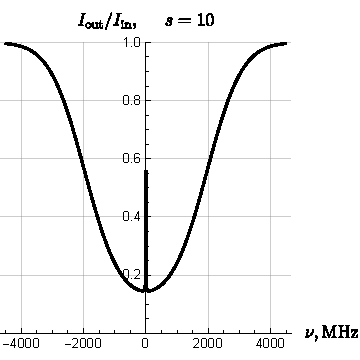
\includegraphics[width=0.33\textwidth]{"D:\\Kami\\git_folder\\notes_5sem\\rqc\\saturation_spectr_simulation\\frac2.pdf"}
    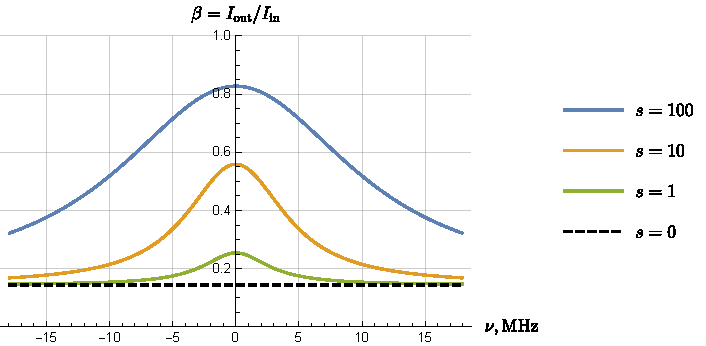
\includegraphics[width=0.63\textwidth]{"D:\\Kami\\git_folder\\notes_5sem\\rqc\\saturation_spectr_simulation\\frac1.pdf"}
    \caption{Спектр вблизи $\nu_{\text{рез}}$ при температуре в $300\ {}^{\circ}$С}
    \label{fig:frac12}
\end{figure} \frametitle{Количественная оценка}}
\frame{
% \begin{equation*}
%     \beta(s=0) \overset{\mathrm{def}}{=}  \beta_0 = e^{- \kappa F(0)},
%     \hspace{0.5cm} \Rightarrow \hspace{0.5cm}
%     \kappa = \frac{\ln 1/\beta_0}{F(0)},
% \end{equation*}
% где $1-\beta_0$ -- глубина доплеровского провала.

Контрастность\footnote{
    Отношение высоты лэмбоского пика к глубине доплер. провала.
}  спектроскопии $K$:
\begin{equation*}
    \frac{\sub{I}{out}}{\sub{I}{int}} = \exp\left[
        - \kappa F(s, \nu)
    \right], 
    \hspace{0.5cm} \Rightarrow \hspace{0.5cm}
    K(s)  = 
    \frac{\beta_0^{F(s)/F(0)}-\beta_0}{1-\beta_0},
\end{equation*}
где $\beta \overset{\mathrm{def}}{=}  \sub{I}{out}/\sub{I}{in}$, подразумеваем $\nu = \nu_\text{рез}$, $\beta_0 \overset{\mathrm{def}}{=} \beta(s=0)$.

\begin{figure}[h]
    \centering
    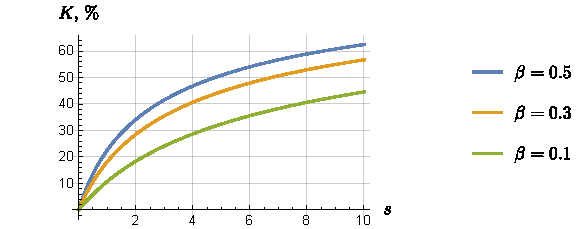
\includegraphics[width=0.81\textwidth]{"D:\\Kami\\git_folder\\notes_5sem\\rqc\\saturation_spectr_simulation\\K.pdf"}
    \caption{Оценка контрастности при различных значениях $\beta$, как функция от $s$}
    %\label{fig:}
\end{figure} \frametitle{Контрастрность спектроскопии}}


\section{Эксперимент}
% установка
\frame{
Диодный лазер сканирует по частотам, близким к 671 нм (D1 и D2 линии ${}^7$Li).

\begin{figure}[h]
    \centering
    \incfig{scheme}
    \caption{Схема установки}
    %\label{fig:}
\end{figure}

При $\omega = \omega_{\text{рез}}$ в резонансе оказываются атомы с нулевой скоростью. \frametitle{Схема установки}}
\frame{
\begin{figure}[h]
    \centering
    \incfig{scheme_photo}
    \caption{Фото установки}
    %\label{fig:}
\end{figure}

 \frametitle{Фото установки}}



% данные
\frame{
Черная кривая -- снятый сигнал, $\cmark$ насыщающий пучок.
Красная кривая -- снятый сигнал, $\xmark$ насыщающий пучок.




\begin{figure}[h!]
    \centering
    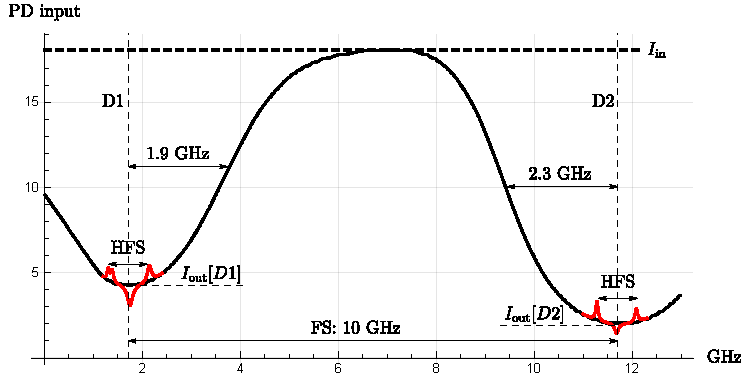
\includegraphics[width=1\textwidth]{D:\\Kami\\git_folder\\notes_5sem\\rqc\\data_processing_1\\exp_D12_v2.pdf}
    \caption{Полученное уширение линий для D1 и D2}
    \label{fig:expD12}
\end{figure}

 \frametitle{Общий вид данных}}
\frame{
Синяя кривая -- фитирование лоренцовым профилем.
Черные точки -- экспериментальные данные.

\begin{figure}[h]
    \centering
    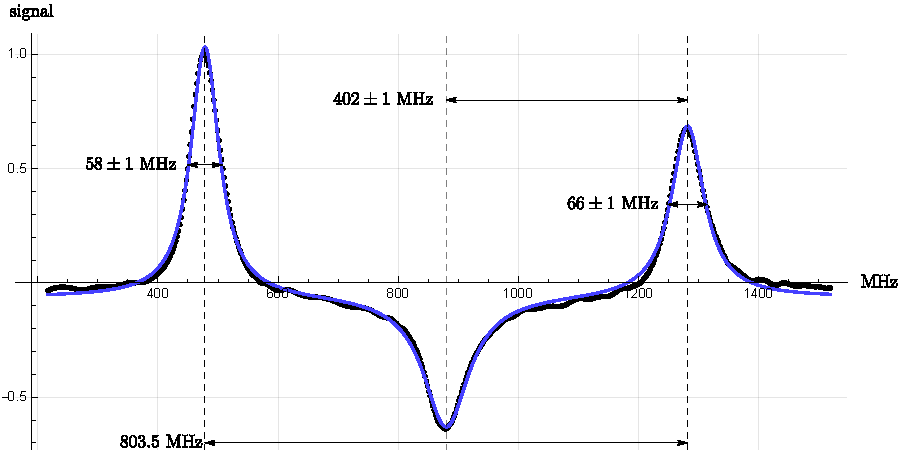
\includegraphics[width=1\textwidth]{D:\\Kami\\git_folder\\notes_5sem\\rqc\\data_processing_1\\exp_D2.pdf}
    \caption{Полученное уширение линий для D${}_2$}
    \label{fig:expD2}
\end{figure}

\vspace{-2mm}
$\Rightarrow$ Наблюдение расщепления $2 \ {}^2\text{S}_{1/2}$: $\Delta \approx 800$ МГц. \frametitle{Линия D${}_2$}}
\frame{
Синяя кривая -- фитирование лоренцовым профилем.
Черные точки -- экспериментальные данные.

\begin{figure}[h]
    \centering
    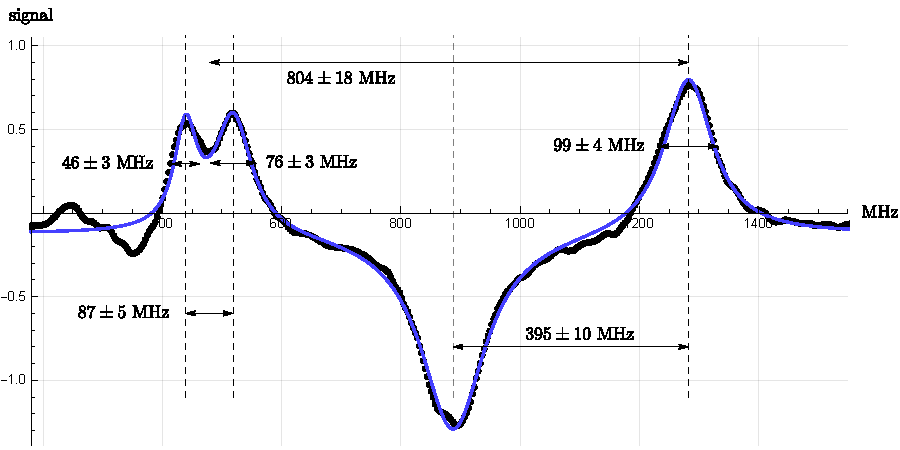
\includegraphics[width=1\textwidth]{D:\\Kami\\git_folder\\notes_5sem\\rqc\\data_processing_1\\exp_D1.pdf}
    \caption{Полученное уширение линий для D${}_1$}
    \label{fig:expD1}
\end{figure}

\vspace{-2mm}
$\Rightarrow$ Наблюдение расщепления $2 \ {}^2\text{P}_{1/2}$: $\Delta \approx 90$ МГц. \frametitle{Линия D${}_1$}}

\section{Результаты}

% выводы
\frame{


\subsection*{Ход работы (шум фактор и темновой счёт)}



\textbf{Частота темнового счёта SiPM}.
Перейдем в режим регистрации экстремумов (рис. 2), и установим временное разрешение в 80 ns. Измерим частоты темнового счёта с различным разрешением res (см. таблицу 1). 


 Построим зависимость (см. рис. \ref{fig:1}) частоты темнового счёта $f$ от разрешения peak-detect,
где $f$ можем найти, как
\begin{equation*}
    f = \frac{\text{hits}}{\text{wfms} \times T},
\end{equation*}
где wfms -- количество разверток, hits -- количество зарегистрированных импульсов, $T$ -- время развертки осциллографа, равно $0.1$ ms.

\begin{figure}[h]
    \centering
    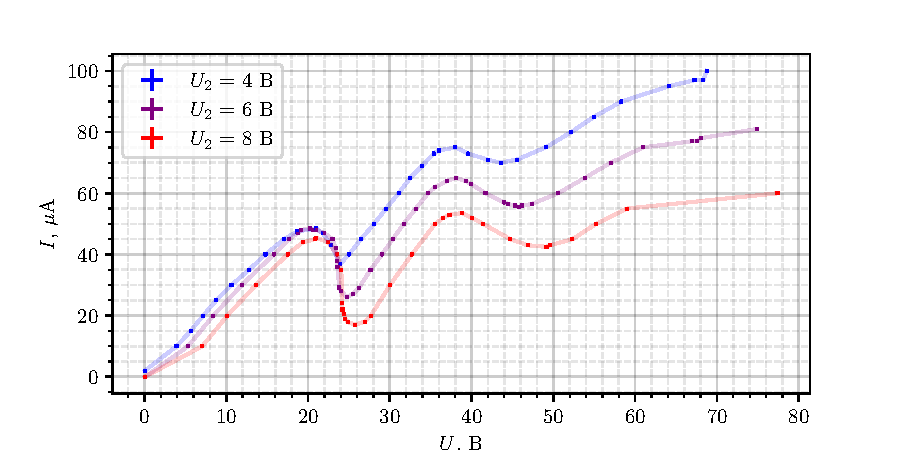
\includegraphics[width=0.75\textwidth]{figures/plot1.pdf}
    \vspace{-5mm}
    \caption{Зависимость частоты темнового счёта $f$ от разрешения res}
    \label{fig:1}
\end{figure}

Можно явно разделить зависомость $f(\text{res})$ на две области, разграниченные значением в $1 \ \mu$с. Чем меньше res, тем чаще импульсы попадают на границу дух временных интервалов, от чего эффектиное значение $f$ увеличивается. Чем больше res, тем чаще неcколько импульсов попадает в один интервадл, от чего эффективное значение $f$ уменьшается. 

Таким образом res $ = 1 \ \mu$с находится в промежутке между длительностью одного импульса и средним периодом повторения, а значит искомое значение частота темнового счёта:
\begin{equation*}
    f = (0.17 \pm 0.02) \text{ МГц}.
\end{equation*}


\textbf{Шум фактор SiPM}. 
Для расчета шум-фактора воспользуемся формулой
$$
F = 1 + \frac{\sigma^2}{\mu^2} = 1.026,
$$
где параметры взяты из гистограммы для разрешения 200\,нс. Из $\sigma$ дополничтельно вычтена $\sigma_\text{sys}$.




\textbf{Оценка величины заряда}
Оценить можно тремя способами.
Во-первых, зная темновой ток и частоту темнового счета $f$ имеем:
$$
q = \frac{I_\text{dark}}{f} = (3.1\pm 0.4)\times 10^{-14}\,\text{Кл} = (1.9\pm 0.2)\times  10^5\, e,
$$
где $e$ -- заряд электрона. 
Во-вторых, исходя из формы пика (рис. \ref{fig:0}) и внутреннего сопротивления осциллографа $R=50\,\text{Ом}$:
$$
q = \frac{1}{R}\int\limits_\text{pike} U(t) \d t \approx \frac{1}{R} \times \text{high} \times  \text{width} = 
\frac{1}{50 \ \Omega} \times  (20 \, \text{мВ})\times (2\, \text{ns}) \approx  5 \times  10^6 e.
$$
В третьих, из прошлой работы известно, что по порядку величины емкость фотодетектора $C \approx 20\,\text{пФ}$, откуда:
$$
q \approx C \cdot \mu = 5\cdot 10^{-13}\,\text{Кл} = 3 \cdot 10^6\, e.
$$
Стандартные отклонения могут быть получены из отклонения амплитуды импульсов:
$$
\frac{\sigma_q}{q} = \frac{\sigma}{\mu} = 0.16.
$$ \frametitle{Выводы}}

% \frame{
% Пока что, в контексте выбранной модели, хуже всего можем оценить $l$, поэтому будем сравнивать теоритескую и экспериментальную оценку $\kappa$ по значению $l$  при котором они бы сходились:
\begin{equation*}
    l = \underbrace{\frac{\log 1/\beta_0}{F[0, \nu_0]}}_{\kappa} \frac{\sqrt{\pi}}{n \sigma_0} \underbrace{\sqrt{\frac{2 \sub{k}{Б} T}{m}}}_{v_0}.
\end{equation*}
Считая $\sigma_0 = \sigma_0^{\text{теор}}$, построим зависимость $l[\beta]$, рис. \ref{fig:lx}.

\begin{figure}[h]
    \centering
    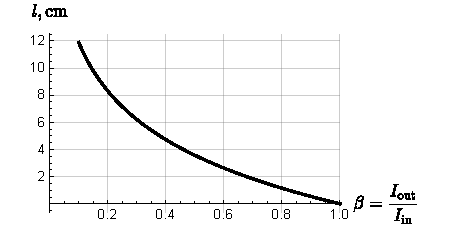
\includegraphics[width=0.5\textwidth]{"D:\\Kami\\git_folder\\notes_5sem\\rqc\\saturation_spectr_simulation\\lx.pdf"}
    \caption{Оценка длины взаимодействия лазера с литием при температуре в $300\ {}^{\circ}$С}
    \label{fig:lx}
\end{figure}
 \frametitle{Дополнение}}


\end{document}



% сделать котов разных цветов
% разобраться с разными headlines
% 